\documentclass[10pt,twocolumn,letterpaper]{article}

\usepackage{cvpr}
\usepackage{times}
\usepackage{epsfig}
\usepackage{graphicx}
\usepackage{amsmath}
\usepackage{amssymb}

% Include other packages here, before hyperref.

% If you comment hyperref and then uncomment it, you should delete
% egpaper.aux before re-running latex.  (Or just hit 'q' on the first latex
% run, let it finish, and you should be clear).
\usepackage[breaklinks=true,bookmarks=false]{hyperref}

\cvprfinalcopy % *** Uncomment this line for the final submission

\def\cvprPaperID{****} % *** Enter the CVPR Paper ID here
\def\httilde{\mbox{\tt\raisebox{-.5ex}{\symbol{153}}}}

% Pages are numbered in submission mode, and unnumbered in camera-ready
%\ifcvprfinal\pagestyle{empty}\fi
\setcounter{page}{1}
\begin{document}

%%%%%%%%% TITLE
\title{Pedestrian Detection Using Correlated Lidar and Image Data \\
      EECS442 Final Project Fall 2016 }

\author{Samuel Rohrer\\
University of Michigan\\
{\tt\small rohrer@umich.edu}
% For a paper whose authors are all at the same institution,
% omit the following lines up until the closing ``}''.
% Additional authors and addresses can be added with ``\and'',
% just like the second author.
% To save space, use either the email address or home page, not both
\and
Ian Lin\\
University of Michigan\\
{\tt\small tiannis@umich.edu}
}

\maketitle
%\thispagestyle{empty}

%%%%%%%%% ABSTRACT
\begin{abstract}
  Recent progress in software and hardware systems will lead to an increase in
  daily interactions with robots and intelligent systems. As a result of this,
  safety must be at the forefront of the design of autonomous systems and
  particularly autonomous cars. Avoiding pedestrians is one of the most important
  aspects of autonomous vehicle safety. With this in mind we aim to create a pedestrian
  detection system based off of sensors commonly found on autonomous vehicles.
  We will use correlated Lidar and image data along with algorithms found in
  recent papers to perform pedestrian detection.

\end{abstract}

%%%%%%%%% BODY TEXT
\section{Introduction}

  As progress in software and hardware continues, it is expected that
  autonomous robotics and intelligent systems will begin to play an integral
  role in everyday life. Jobs that are physically demanding or unsafe can be
  replaced by robots. Autonomous cars can greatly improve road safety and
  efficiency, as most traffic accidents today are a direct result of human error.
  In order for these intelligent systems to succeed, they must be designed
  to be safer than a human driver. Obstacle detection is a crucial aspect
  of this - especially for autonomous cars which
  must detect other cars, road signs, traffic signals, and
  pedestrians. Beyond just detecting obstacles, it is often necessary
  to predict the future motion of moving obstacles such as other vehicles,
  pedestrians, and animals. We aim to focus our efforts on detecting the presence
  of pedestrians in both Lidar (light
  detection and ranging) scans and images.

  The goal of this project is to detect pedestrians in a pre-existing dataset:
  the Laser and Image Pedestrian Detection (LIPD) dataset \cite{dataset},
  which provides correlated Lidar and image data. We aim to identify pedestrians
  on the road based on Lidar data by first segmenting the scans and then 
  extracting features from those segments.
  After feature extraction, we plan to use a trained classifier to determine
  if the obstacle is indeed a pedestrian in the road. Then we plan to extract
  pedestrian features from the images using OpenCV \cite{opencv}. We could extend this by
  training a more sophisticated classifier that has the ability to discern the
  difference between cars, pedestrians, and road signs based on both Lidar
  and image data.

%------------------------------------------------------------------------
\section{Previous Work}

  There has been a good deal of work in the area of pedestrian detection for
  mobile robotics. In most systems, the sensor subsystems operate independently
  of each other. In \cite{journal} the authors used Lidar data to generate regions
  of interest, then use image analysis to determine whether a pedestrian is
  present. Some other sensors available on modern autonomous robotics
  platforms include: radar, ultrasound, cameras, and Lidar. However, 
  each of these sensors comes with their own
  inherent problems. Cameras can fail in low light situations and Lidar can
  fail when objects are side by side at the same distance. Both can fail in poor
  weather: Lidar if rain or snow causes the light to be reflected
  too early and cameras if the lens is obstructed by snow or fog.

  In order to complete this project, we started with the LIPD dataset \cite{dataset}.
  Some benefits of this dataset include: correlated Lidar and image data, pre-segmented
  Lidar scans, features from segmented Lidar scans, and
  a classification dataset. The correlated datasets were composed of a forward
  facing camera (limited field of view relative to Lidar) and four Lidar scans
  all facing outwards at different angles. The classification dataset had both
  training and testing sets for the Lidar data.


%------------------------------------------------------------------------
\section{Technical Work}

  We plan to use both Lidar data and images to identify
  pedestrians on the road. With Lidar data, we can identify obstacles on the
  road and then analyze the corresponding images that potentially contain
  pedestrians to determine if pedestrians are present. There has already 
  been work done in the areas of correlating
  Lidar and single image data for the purpose of detecting pedestrians. Most
  of it follows a similar approach to the one we are outlining and has been successful.
  For Lidar object detection, we decided to follow the pipeline outlined
  in \cite{journal}, and add stages for error correction and comparison with
  OpenCV \cite{opencv} pedestrian detection based on image data. 
  The pipeline is as follows: segmentation, feature
  extraction, classification, error correction, and comparison with image based
  pedestrian detection.

  \subsection{Segmentation}
  The pipeline begins with segmentation of the Lidar data
  to find the points where the directionality of the segment changes.
  According to \cite{conf} if it
  is a new segment then (1) holds true where $r_i$ is the
  distance to current point, $r_{i+1}$ is the distance to next point,
  $cos(\Delta \alpha)$ is the 3D angle between the two points, and $C_0$ is a
  constant to adjust for noise:
   \begin{equation} \sqrt{r_{i}^{2} + r_{i+1}^{2} - 2 r_{i} r_{i+1}
   cos(\Delta \alpha)} > thd \end{equation}
   \begin{equation} thd = C_0 + \sqrt{2(1-cos(\Delta \alpha}) * min(r_i,
   r_{i+1}) \end{equation}

   \begin{equation}  cos(\Delta \alpha) = \frac{r_i \cdot r_{i+1}}
   {||r_i||||r_{i+1}||} \end{equation}

  For the purpose of this project any segment less than three points long was
  discarded before moving to feature extraction. This was performed for each
  Lidar scan in isolation of the other scans.

  \subsection{Feature Extraction}
  After separating the Lidar scan data into different segments we then
  performed feature extraction on the segments. We used 10 different features
  for each segment, based on \cite{journal}.

  \renewcommand{\arraystretch}{1.5}
  \begin{center}
    \begin{tabular}{ | p{1cm} | l | p{2.9cm} |}
      \hline
      Feature num & Formula & Description \\ \hline
      1 & $ np $ & number range points \\ \hline
      2 & $np*r_{min}$ & number of range points * minimum range distance \\ \hline
      3 & $\sqrt{ \Delta X^2 + \Delta Y^2} $ & RMS of segment width and height
      \\ \hline
      4 & $ \frac{1}{np}\sum_{n=1}^{np} || x_n - x_m|| $ & Mean average deviation
      from median ($x_m$) \\ \hline
      5 & $ \frac{1}{np}\sum_{n=1}^{np} (x_n - x_{lsq})^2 $ & Linearity -
      distance to the least squares line ($ x_{lsq}$) \\ \hline
      6 & $ \frac{1}{np}\sum_{n=1}^{np} (x_n - \mu_x)^2 $ & Second central
      moment (about mean $\mu_x$) \\ \hline
      7 & $ \frac{1}{np}\sum_{n=1}^{np} (x_n - \mu_x)^3 $ & Third central
      moment (about mean $\mu_x$) \\ \hline
      8 & $ \frac{1}{np}\sum_{n=1}^{np} (x_n - \mu_x)^4 $ & Fourth central
      moment (about mean $\mu_x$) \\ \hline
      9 & $ \sum_{n=1}^{np} ||x_n - x_{n-1}|| $ & Segment length (norm distance
      between points) \\ \hline
      10 & $ \sigma(ft9) $ & Standard deviation of
      segment length (norm distance between points) \\ \hline
    \end{tabular}
  \end{center}

  These features describe the distribution of segment points and were all
  computationally cheap and robust for all segments greater than three points long.

  \subsection{Classification}
  For classification we used training data from \cite{dataset} to train a Python
  SkLearn DecisionTreeClassifier \cite{sklearn}. The training data consisted of
  pre-segmented Lidar scans that were very clean and well segmented. The Lidar
  scans were split between segments with pedestrians and segments without
  pedestrians. A similar set of test data was also provided and our classifier
  achieved an accuracy of 88\%.

  \subsection{Error Correction}
  Since our Lidar data consists of four horizontal scans taken at slightly different angles,
  we should expect that the existence of pedestrians results in several positive segment
  classifications (up to four) in the same area. Therefore, a simple way to decrease
  the number of positive classifications is to only positively classify segments if there
  are other segment classifications in agreement within a small pixel margin.
  Taking Figure 1 for example, we get a large number of segments on the right side
  of the image around the two women which would be saved since there are many segments in
  agreement vertically. However, some of the other false positives would be ignored
  since as they are more isolated.

  To do this error correction, we first classify and store all of our positive segments. For each
  segment, we then check if the other scans contain positive segments within a threshold
  of the original segment. If there are no other segments that corroborate
  the positive classification of the original segment, then we do not consider it a positive
  segment and remove it from our output. We have a large degree of flexibility in
  this filtering process as we can both vary the threshold as well as the number of segments
  in agreement. We found that a threshold $ thd = 10 $ and a single additional segment in
  agreement appeared to give good results. Requiring more segments to agree or using a lower
  threshold results in over-filtering whereas a larger threshold would not filter enough
  false positives out.

%------------------------------------------------------------------------
  \begin{figure}
    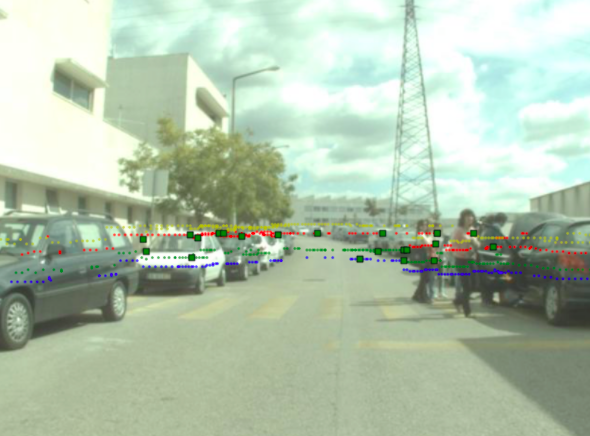
\includegraphics[height=2.8in, width=3.5in]{images/initial_result.png}
    \caption{ Initial segmentation results. Green squares are identified
    segments. Red, blue, yellow and green dots are Lidar points.}
  \end{figure}
\section{Experimental Results}
  We ran our pipeline on raw Lidar scans correlated with image data. After
  segmenting each of the four Lidar scans individually, we pass each segment to the
  feature extractor. The feature extractor outputs a feature vector composed of
  the ten features described above and our classifier is able to make a binary
  classification of whether or not the segment contains a pedestrian. To visually
  display our results, we overlay each of the four Lidar scans over its corresponding
  image. We color each Lidar scan a different color --yellow, red, green, and blue--
  to distinguish between them. Since the Lidar scan is wider than the image,
  we do not display Lidar points beyond the width of the image. Segments that are
  positively classified as pedestrians are saved. Their start and end are plotted
  as large green squares.

  \subsection{Example Lidar Output}
  An example of the output of our system can be seen in Figure 1. Our Lidar
  classifier does pick up the two women on the right side of the image as two
  distinct pedestrians. There are additional people behind these two women
  who are largely occluded and are not identified by our classifier. Unfortunately
  we also get several false positives around the cars on the left side of the road.

  \begin{figure}
    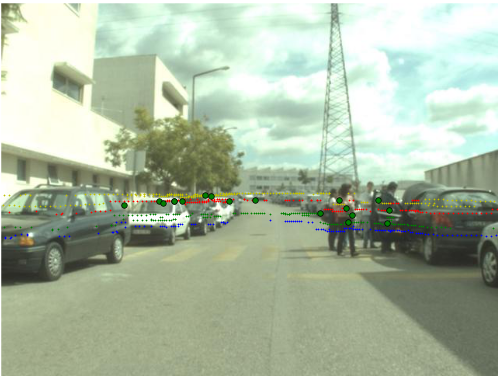
\includegraphics[height=2.8in, width=3.5in]{images/filterSampleOriginal.png}
    \caption{ Unfiltered Example. Green squares are identified
    segments. Red, blue, yellow and green dots are Lidar points. Notice the
    amount of false positives in the left and center regions of the image.}
  \end{figure}


  \subsection{Example Lidar output after Filtering}

  Shown in Figure 2 is another unfiltered image very similar to Figure 1. As you can see,
  there are several false positives on the left side and center regions of of the image.
  These false positives are mostly isolated while the correctly classified pedestrian
  region has many segments in agreement.

  Figure 3 is the result of our Lidar scan after filtering out segments
  that were not present in multiple Lidar scans. On the left side of the image
  approximately five incorrect Lidar points were removed and in the center of
  the image another five incorrect Lidar points were removed. This demonstrates that
  our filtering algorithm is clearly working in this case, as it removes many
  of the false positives. Furthermore, we can tune this algorithm to work
  even better by adjusting the threshold of how close segments must be,
  accounting for segment length, and modifying the number of segments required for
  agreement. For example, Figure 3 still contains false positives even after filtering:
  there is a small cluster of green squares on the tip of the black car on the left
  side. Raising the number of segments necessary for a positive classification from two
  to three would likely fix this issue (but may cause false negatives in other examples).

  \begin{figure}
    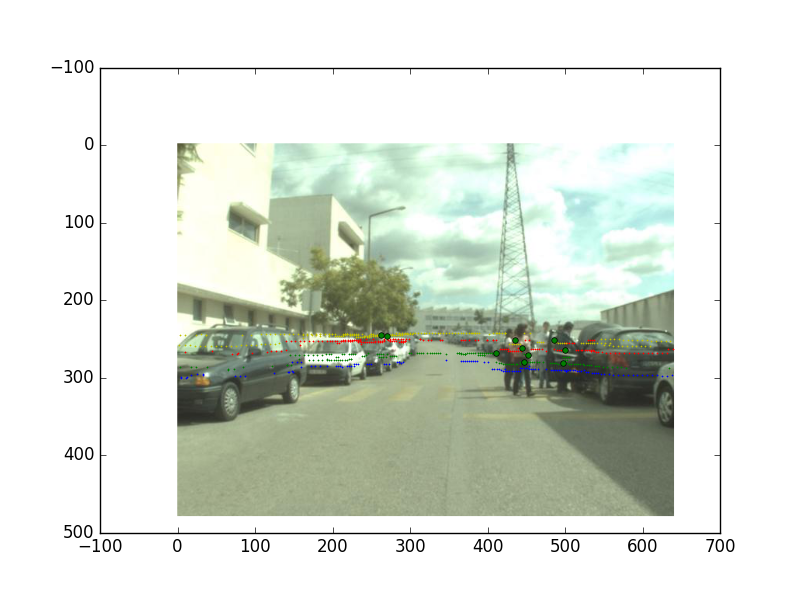
\includegraphics[height=2.8in, width=3.5in]{images/filterSampleResults.png}
    \caption{ Segmentation results after filtering. Green squares are identified
    segments. Red, blue, yellow and green dots are Lidar points. Notice the
    amount of false positives removed from Figure 2 in the left and center
    regions of the image.}
  \end{figure}


  \subsection{Example OpenCV Output}
  An example of the output of OpenCV's PeopleDetect \cite{opencv} code can be seen in Figure 2.
  The results are surprisingly similar to our Lidar classifier: it picks up the two
  women as well as two extra false positives. The output of OpenCV is more clearly
  indicated than the output of our Lidar scans as they can draw very nice bounding
  boxes around the pedestrians. Unfortunately Lidar scans do not provide any height
  information that can be extrapolated so estimated bounding boxes would have to be
  drawn with some assumption regarding the average height of a pedestrian.

  \begin{figure}
    \includegraphics[height=2.8in, width=3.5in]{images/peopledetect.png}
    \caption{ Example output of OpenCV's PeopleDetect \cite{opencv}. }
  \end{figure}


  \subsection{OpenCV PeopleDetect vs. Lidar Classifier}
  In general both OpenCV's PeopleDetect \cite{opencv} and our Lidar Classifier were
  able to identify regions with pedestrians. However, our Lidar Classifier tended to
  make many more false positive classifications than PeopleDetect. There are both
  cases where our Lidar Classifier performs better than PeopleDetect and cases where
  PeopleDetect performs better than our Lidar Classifier. An example of where PeopleDetect
  fails to pick up any pedestrians and makes two false positives can be seen in Figure 6.

  The same image with our Lidar Classifier, see Figure 5, does pick up the group of pedestrians but again
  makes several false positive classifications. However, this image did not incorporate our
  filtering step mentioned above which likely would have removed most of the false positives.
  In this particular case, our Lidar Classifier does much better than PeopleDetect but this
  demonstrates the difficulty in merging Lidar and Image classifications. There will be cases
  where the classifications are in agreement but there will also be cases like this where there
  is no overlap.

  \begin{figure}
    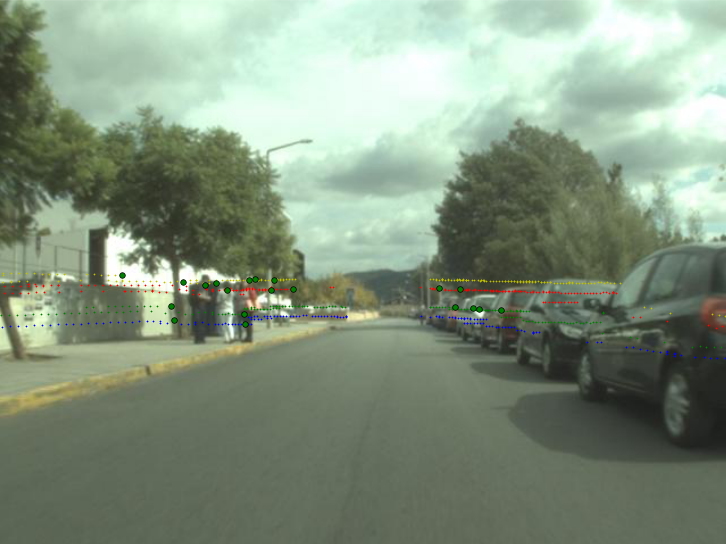
\includegraphics[height=2.8in, width=3.5in]{images/sample2lidar.png}
    \caption{ Pedestrians identified by Lidar Classifier and filtering shown
    by green squares. Notice correct identifications of pedestrians. }
  \end{figure}

    \begin{figure}
    \includegraphics[height=2.8in, width=3.5in]{images/sample2cv.png}
    \caption{ Pedestrians identified by OpenCV PeopleDetect \cite{opencv}.
    Notice the two false positives found and that the actual pedestrians are
    not detected. }
  \end{figure}

%------------------------------------------------------------------------
\section{Future Work}
  As seen in Figure 1 and mentioned above, our Lidar classification does output a
  large number of false positives. While this is somewhat better than false negatives--
  identifying too many pedestrians is preferable over missing one--we believe that
  our results could be improved by minimizing false positives and more closely
  tying image classifications with our Lidar classifications.

  \subsection{Correlation with Image Data}
  We could improve our results by making a final prediction that combines
  results of both the Lidar classification and image classification. A simple
  set intersection of the general areas where the positive Lidar segments and OpenCV
  bounding boxes are in agreement could cut down on the extra classifications coming from
  both our Lidar Classifier as well as OpenCV's PeopleDetect. See Figure 7 for an example of a potential
  output of such a system that combines the Lidar Classifier output from Figure 1
  and the PeopleDetect output from Figure 4. As you can see
  the simple set intersection removes the false positives stemming from both OpenCV and
  our Lidar Classifier.

  However, there are many difficulties in combining the two systems once you look
  beyond just this image. As mentioned above, it is unlikely the systems will always
  agree as seen with Figures 5 and 6. A simple set intersection could well likely result
  in no positive classifications and many false negatives which would be disastrous
  for an autonomous vehicle. A safer choice would be a set union between the two as
  false negatives are far worse than false positives.

  \begin{figure}
    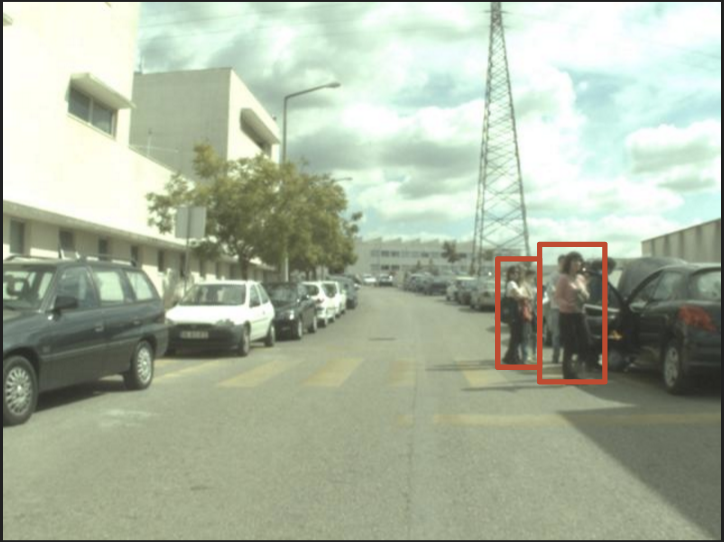
\includegraphics[height=2.8in, width=3.5in]{images/futureWork.png}
    \caption{ Example output of potential system that combines a Lidar Classifier 
    with OpenCV PeopleDetect \cite{opencv}. Bounding boxes are hand-drawn. }
  \end{figure}

%------------------------------------------------------------------------
\section{Conclusion}
  We were able to segment raw Lidar scans, extract
  features, and make a successful pedestrian classification. 
  Unfortunately the final dataset that
  we tested our system on provides labels as a series of bounding boxes on the
  image itself. As such, we did not have labels for individual segments and do
  not have an exact accuracy for our classifier. However, our initial examination
  of results does look fairly positive: we generally do pick up pedestrians
  but also pick up other objects on the side of the road such as cars.

  Addition of the OpenCV PeopleDetect \cite{opencv} code provides additional interesting
  results. Similarly to our Lidar Classifier, OpenCV does generally detect
  pedestrians but also provides incorrect bounding boxes around cars and buildings.
  These incorrect classifications generally do not coincide with our Lidar
  classifications and thereby validates our initial beliefs that a system combining
  both Lidar and Image classifications can perform better than either individually.

%------------------------------------------------------------------------

{\small
\bibliographystyle{ieee}
\bibliography{egbib}
}

\end{document}
